%!TEX root=paper.tex

\newpage
% \section{How Is Reader Personalization Being Used?}
\section{How Is Reading Personalization Being Used?}
% \section{How Do Learners Use Reader Personalization?}
% \section{How Do Students Use the Possibility of Reading Personally Interesting Articles?}
\label{sec:results}


% \subsection {Feed Subscriptions}
Figure \ref{fig:subscriptions} represents an incidence matrix in which the columns represent students and the rows represent article sources. If at the end of the study a student is registered to a given source, the intersection of the respective row and column has a $\Diamond$. 
% 
We would expect to see fully continuous horizontal rows of data-points if every user subscribed to the same feed, and fully continuous vertical rows if every user subscribed to all of the feeds available. The fact that these patterns are largely absent in Figure \ref{fig:subscriptions} supports our assumption that different individuals prefer to subscribe to different reading sources.

% The figure illustrates that giving the students the freedom to choose the sources they wanted, allowed each one of them to express their interest. 

\begin{figure}[h!]

\centering
  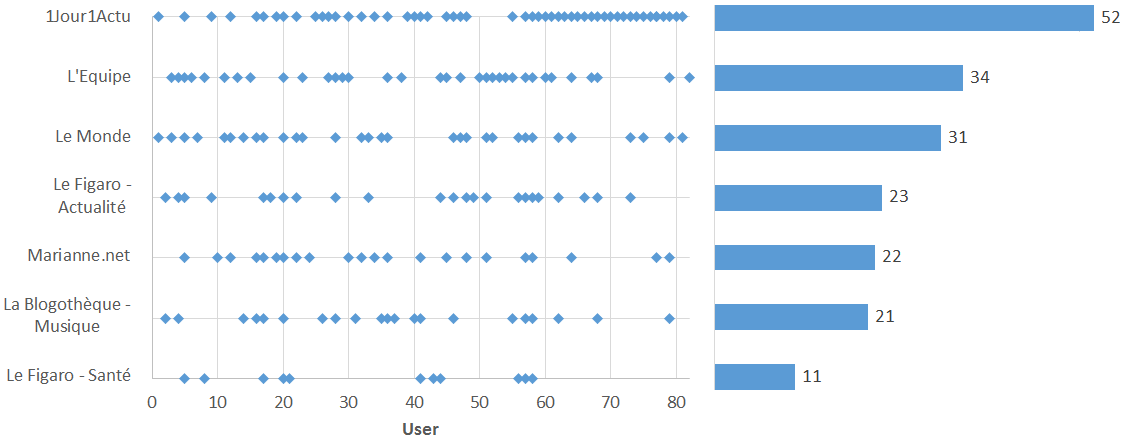
\includegraphics[width=0.9\columnwidth]{figures/subscription_plot}
  \caption{Different students subscribe to different sources}
  \label{fig:subscriptions}  
\end{figure}

The histogram to the right of Figure \ref{fig:subscriptions} shows that some feeds are more popular than others. 
% Projecting the data- points onto the horizontal axis and sorting the results results in the histogram in Figure \ref{fig:feedpopularity}.
% 
% \begin{figure}[h!]
% \centering
%   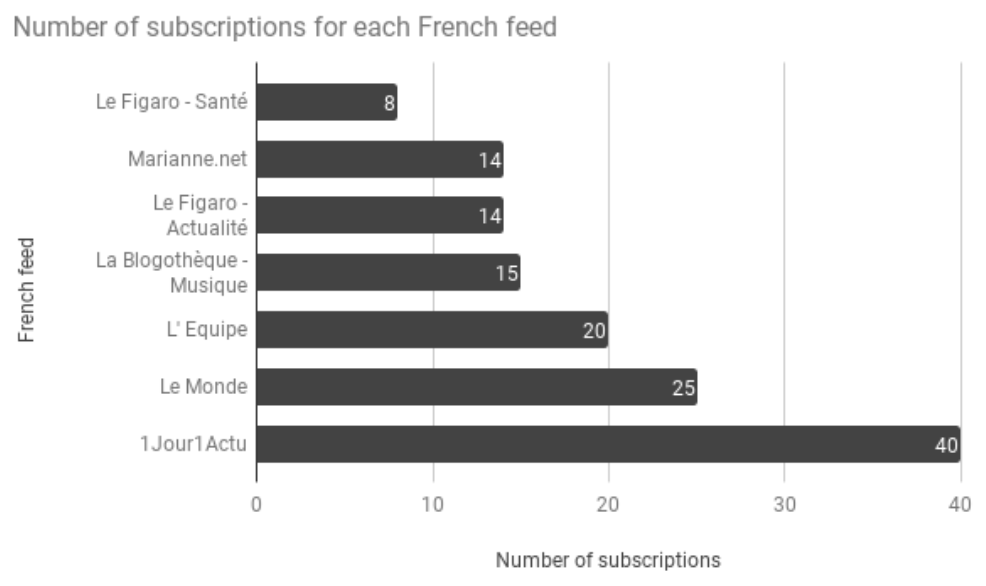
\includegraphics[width=0.85\columnwidth]{figures/feed_popularity}
%   \caption{Some feeds are more popular than others}
%   \label{fig:feedpopularity}
% \end{figure}
% {\em 1Jour1Actu} is the most popular article source and Le Figaro - Sant\'e is the least. 
In order to see whether or not this might be related to how they are presented in the dialog window of our system (Figure \ref{fig:system_subscriptions}), Figure \ref{fig:popularityvsranking} compares the order of popularity with the order in which they are displayed. 
% One can see how the second-to-last presented feed, Le Monde, is the second most popular feed by measure of subscriptions. Conversely, the feed listed above Le Monde is actually the least subscribed-to feed in our listing.


\begin{figure}[h!]
\centering
  \newcommand{\picscale}{0.5}
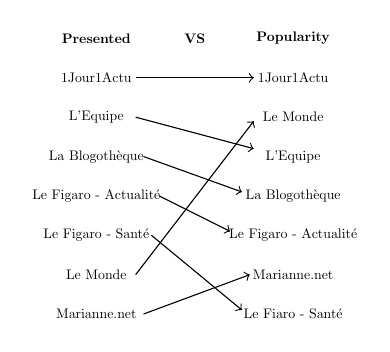
\begin{tikzpicture}[scale=\picscale, every node/.style={scale=\picscale}]
    % Columns.
    \node at (0  , 0) {\bf Presented};
    \node at (2.5, 0) {\bf VS};
    \node at (5  , 0) {\bf Popularity};
    
    % As presented.
    \node at (0,-1) {1Jour1Actu};
    \node at (0,-2) {L'Equipe};
    \node at (0,-3) {La Blogoth\`{e}que};
    \node at (0,-4) {Le Figaro - Actualit\'{e}};
    \node at (0,-5) {Le Figaro - Sant\'{e}};
    \node at (0,-6) {Le Monde};
    \node at (0,-7) {Marianne.net};
    
    % As popular.
    \node at (5,-1) {1Jour1Actu};
    \node at (5,-2) {Le Monde};
    \node at (5,-3) {L'Equipe};
    \node at (5,-4) {La Blogoth\`{e}que};
    \node at (5,-5) {Le Figaro - Actualit\'{e}};
    \node at (5,-6) {Marianne.net};
    \node at (5,-7) {Le Fiaro - Sant\'{e}};
    
    % Arrows between presented and popular.
    \draw [->] (1,-1)   --   (4,-1);
    \draw [->] (1,-2)   --   (4,-2.8);
    \draw [->] (1.2,-3) --   (3.7,-3.9);
    \draw [->] (1.6,-4) --   (3.4,-4.9);
    \draw [->] (1.4,-5) --   (3.7,-6.9);
    \draw [->] (1,-6)   --   (4,-2.1);
    \draw [->] (1.2,-7) --   (3.9,-6);
    
\end{tikzpicture} 
  \caption{The popularity of the feeds vs. their ranking in the UI}
  \label{fig:popularityvsranking}
\end{figure}



% \subsection{Article Interactions}
Figure \ref{fig:articles_read} shows an incidence matrix of users (columns) and articles that they interact with (rows). It shows that each user explores their own interest.
% , and there is no one article that is interesting for all. 
% The vertical ``line'' in the figure's left half represents an over-active reader.
% \begin{added}
  % Interacting with means that the user translated at least one word in that article. to check with Dan that this is the definition! we currently do not have information about whether a user read the article to the end. 
% \end{added}
% 
% \begin{added}
% 
  % After investigating the reading patterns of students we observed that there are those who enjoy reading a variety of topics, but also those who like to read a single topic. 
  % From the latter category we mention: 
It also shows a few students who read exclusively articles about sports (e.g. the rightmost column), but also a student who reads articles exclusively about health topics. Finally, most of the students read a mix of topics, which is beneficial from a learning point of view \cite{renadya07-power}.
  % \begin{itemize}
  %   \item one student who has read twelve articles exclusively on topics about sports in five different days
  %   \item one student who has read six articles exclusively about health topics over two distinct days
  %   \item TODO: Add discussion about some students who have a more omnivorous taste, and thus, also read much more.
  % \end{itemize} 


    % The student \#657 in the published dataset has read 10 articles exclusively about sport in three different days between June 7 and July 4th. 
  
% \end{added}

\begin{figure}[h!]
\centering
  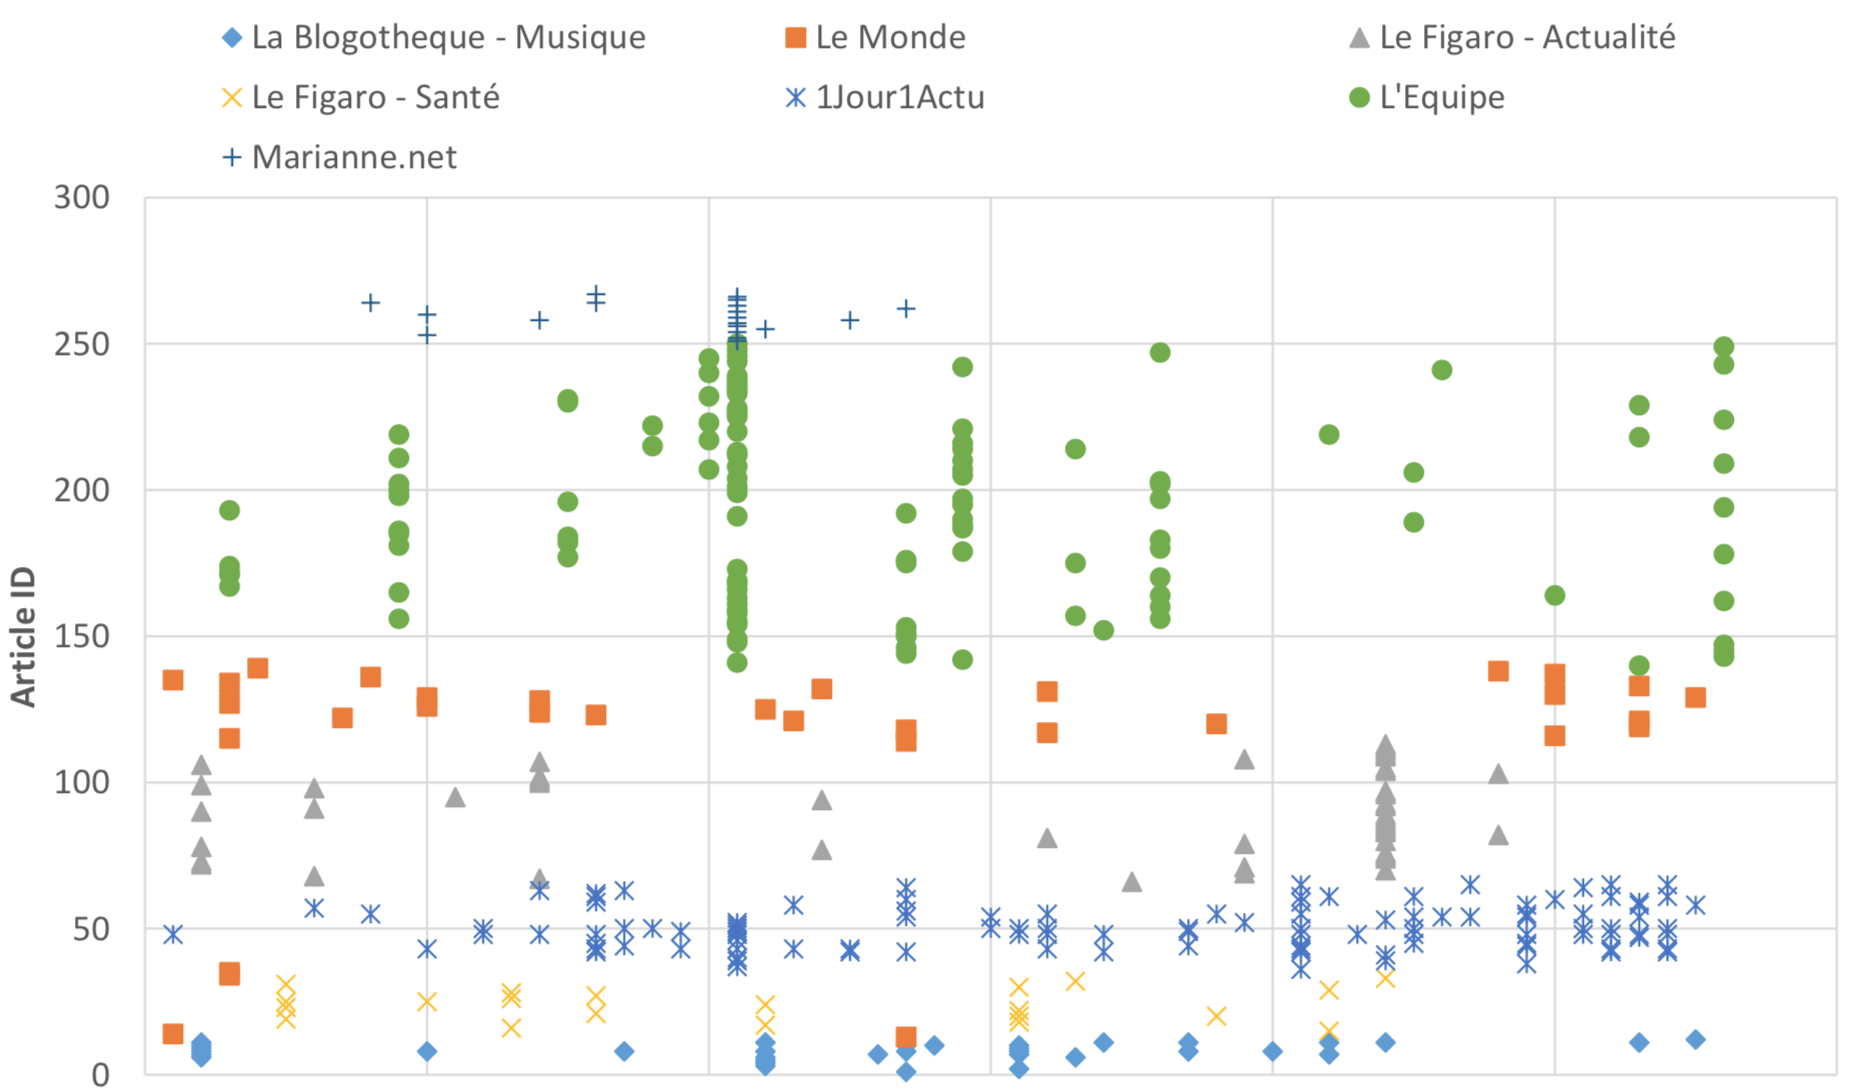
\includegraphics[width=\columnwidth]{figures/users_articles_color_png}
  \caption{Each student (column) reads a different article mix}~\label{fig:articles_read}
\end{figure}


% \newpage
% \section{How Are The Reader Features Used?}
\section{How Do Learners Interact With the Reader?}
% \section{What Is The Relative Importance of the Various Interaction Modes?}
\newcommand{\feature}[1]{{\em #1}}
The reader interaction is more innovative and complex than the exercises.
We use telemetry to investigate how do learners use the features of the reader. 

Telemetry has been successfully used for understanding user behavior in games \cite{Gagne11-telemetry} but also more generic contexts, such as automatically detecting personas from large scale interaction data \cite{Zhang16-telemetry}. In our study, we used telemetry to track the usage of various relevant features in the reader of the personalized textbook in order to better understand the usage of our system.

Based on logging every interaction of every user, Figure \ref{fig:feature_usage} (left) shows the six most used features of the system.\footnote{An extended analysis that includes more features is elsewhere. \cite{Chirtoaca17-apollo}} Figure \ref{fig:feature_usage} (right) shows the number of distinct users for each category of events. A larger number of distinct users indicates a feature that is more important to the students. 

  \begin{figure}[h!]
  \centering
    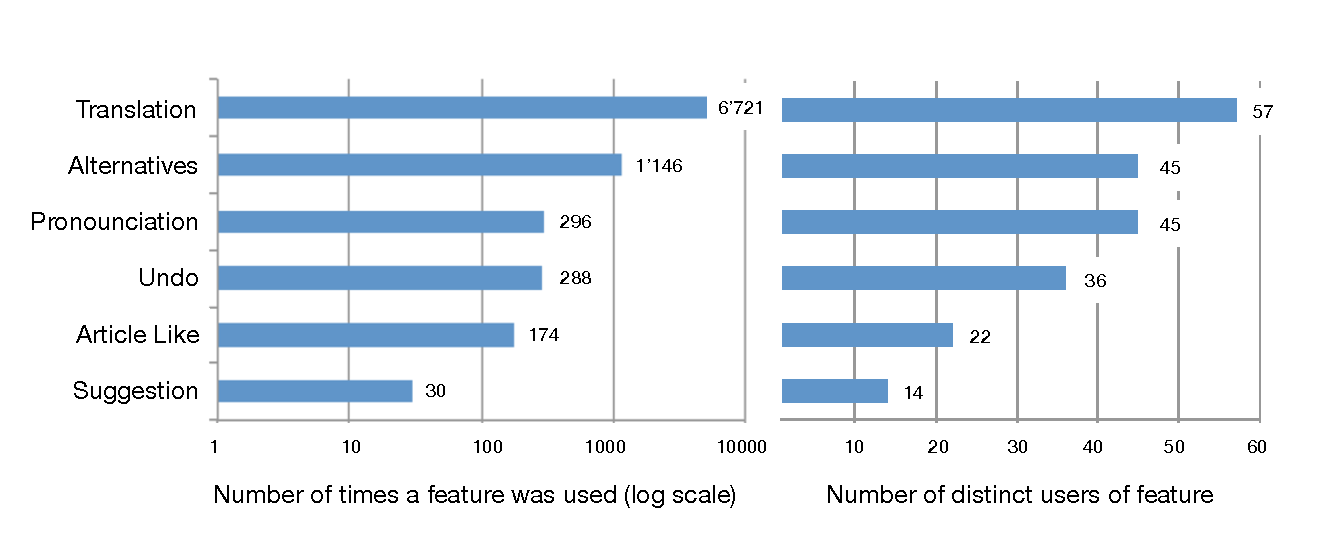
\includegraphics[width=1.0\columnwidth]{figures/feature-usage}
    \caption{Popularity of features by their recorded usage-events}
    \label{fig:feature_usage}
  \end{figure}

% With 6.700 occurrences, 
\feature{Requesting a translation} is the most used feature of the system and \feature{showing translation alternatives} is the second most used one. The six-to-one ratio between the two features is an indicator of the limitations of the automatic translation. The fact that they are both achievable with one click or touch proves to have been a good decision. 
 % -- these are probably the situations when learners ask for 

\feature{Pronuncing a word} is he third most used feature. On average, there are about 1.66 pronunciations for a given translation, suggesting that users are often asking for a second pronunciation after hearing it the first time. 

% \ml{@dan, do you agree with this conclusion? it's opposite to your thesis, but I think this is the correct interpretation}

% In addition, we looked at the number of times the same word or phrase was pronounced by the same user. This data ranges from one single pronunciation to 14 pronunciations for the same word (phrase). The size of this interval is mostly due to the users' different proficiency in a certain language and the difficulty in pronunciation of the word (phrase) itself. Nevertheless, on average, the number approaches 1.66 pronunciation requests for the same piece of text, suggesting that users are generally sufficiently content with a pronunciation after hearing it the first time.


\feature{Undo-ing a translation} is used when the user wants to remove the last translation that was inserted in the text. For the proposed interaction mechanism this feature seems useful. 

\feature{Liking} an article that was just read by clicking the corresponding button at the bottom of an article happened 174 times. This information can be used in the future to improve article recommendations.
 % and maybe to add a social dimension to the system by providing information about how other people react to a given article.

\feature{Suggestion} is a feature that is used seldom and by only a minority of users. This feature, allows users to contribute their own translations when they are not satisfied with the one automatically provided by the system. This feature is not only used seldom, it is also used by very few users. It still is to be determined whether this is due to readers overwhelmingly being satisfied with the automatic translations and their alternatives, or due to a low involvement.
% \ml{which brings me to: @Dan, what do you mean by alternatives here? :) Is it the number of times somebody selected an alternative, or the number of times they opened the menu. In any case, can we get the other number?}

  % \begin{figure}[h!]
  % \centering
  %   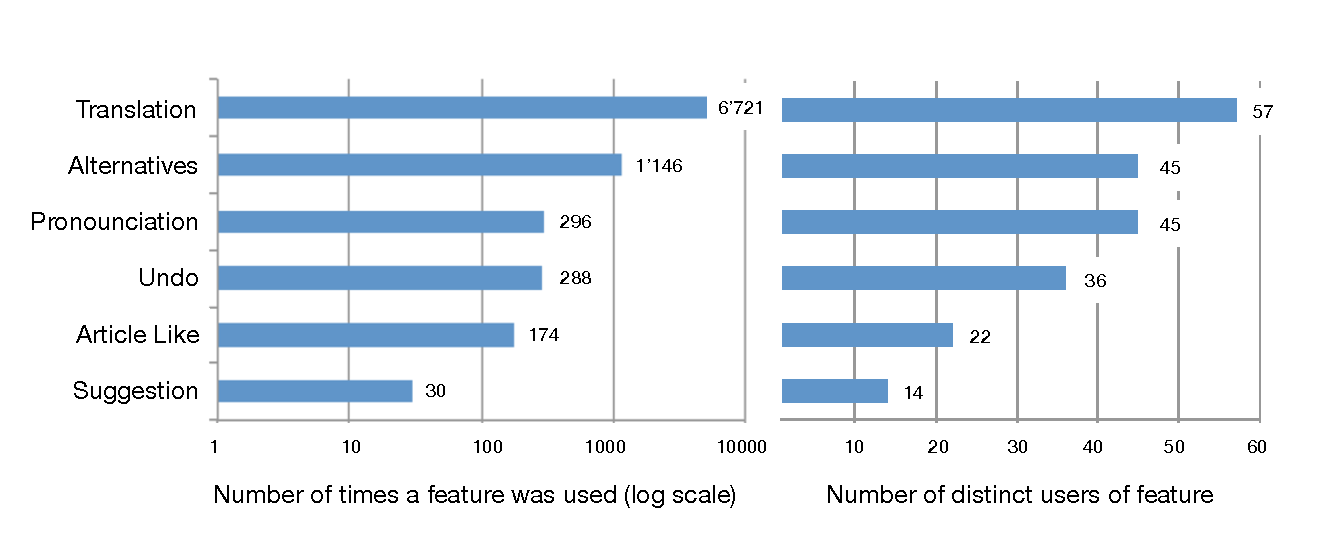
\includegraphics[width=0.6\columnwidth]{figures/feature-usage}
  %   \caption{The usage of the various reader features by the various users }
  %   \label{fig:usage_per_user}
  % \end{figure}


%  We see that: 
% \begin{itemize}
%   % \item Not all the users of the system use translations
%   % \item \feature{Translation suggestion} is used by very few users. It still is to be determined whether this is due to readers overwhelmingly being satisfied with the automatic translations and their alternatives, or due to a low involvement. 
% \end{itemize}




% \newpage
\section{How Do Students Interact With Exercises?}

The system presented four types of vocabulary practice exercises to the students. In total, during the entire duration of the study we observed 18.082 exercises being presented to the students. Figure \ref{fig:ex_interactions} presents the number of exercises which had a ``correct'' outcome (red) vs. exercises which had a ``wrong'' outcome (blue). The figure shows one student who did 3.000 (!) exercises during one month, and about six eager students who did more than 700 exercises. 

  \begin{figure}[h!]
  \centering
    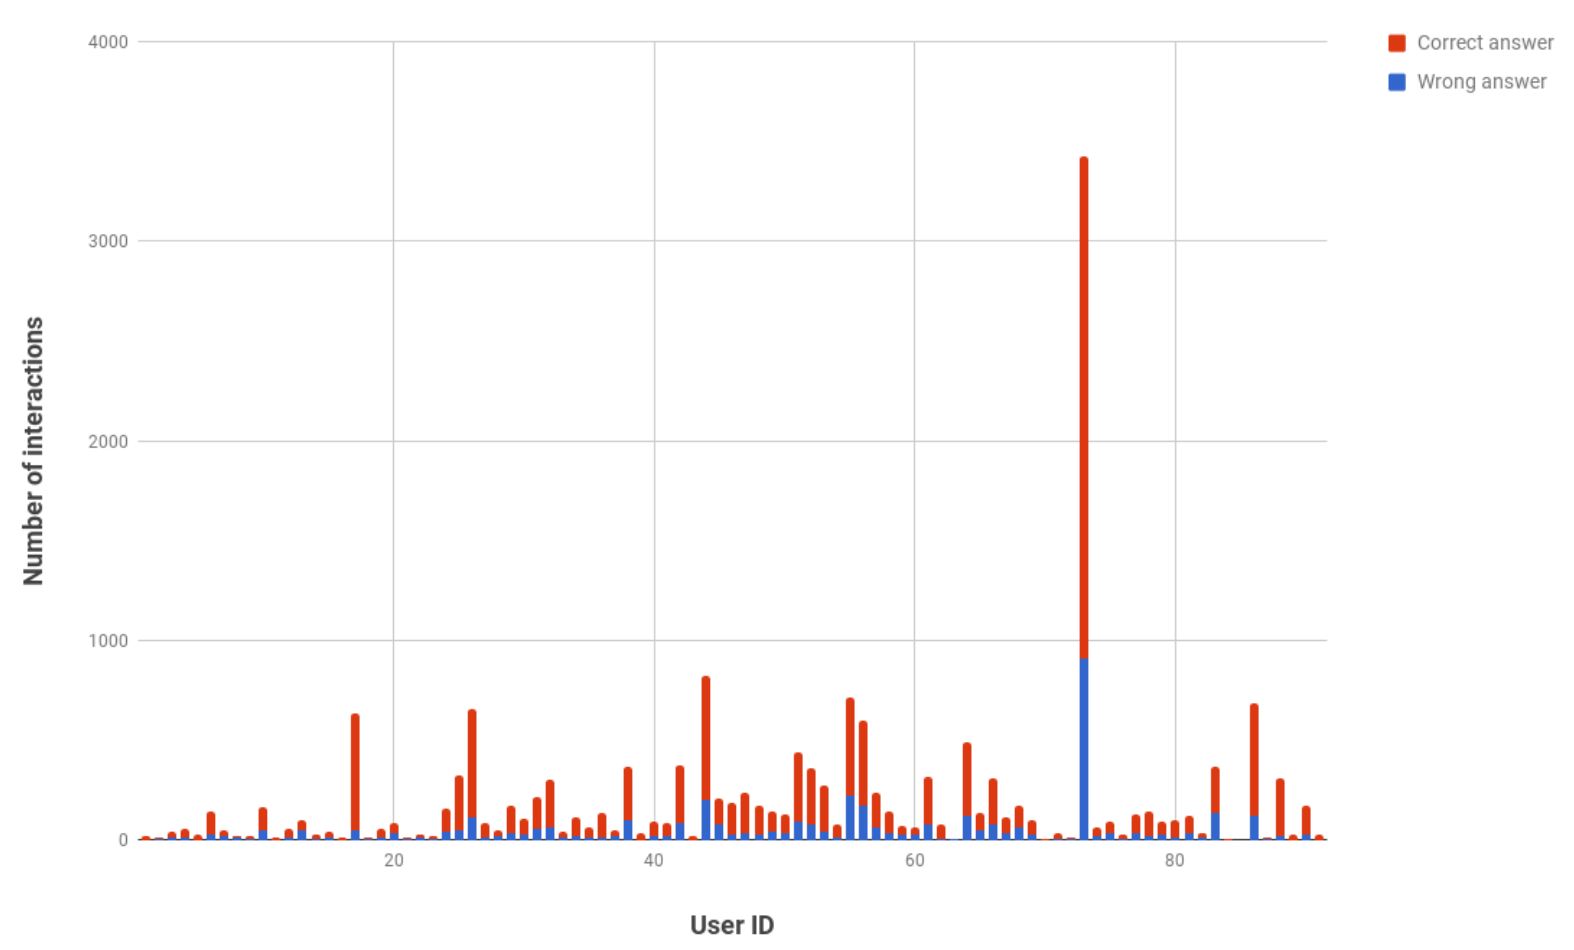
\includegraphics[width=0.9\columnwidth]{figures/exercise_interactions_count.png}
    \caption{Correct (red) and wrong (blue) exercise outcomes per student}
    \label{fig:ex_interactions}
  \end{figure}

The figure does not include one other type of outcome, {\em requesting a hint}, which is presented in the table below grouped per exercise type. The corresponding number of hints suggests that the multiple-choice exercises (i.e. Match, Choose) are simpler than free text entry exercises (i.e. Find, Translate).

\begin{tabular}{lrrrr}
  % source id: 
  % choose -- 5
  % find -- 4
  % translate -- 7
  % match -- 6
                      & Choose  & Find & Translate & Match \\ \hline
  Total interactions  & 7180    & 6249 & 2643      & 2010\\
  Hint requests       & 29      & 529  & 847       & 16 \\ \hline
  \label{tab:hints_per_ex_type}
\end{tabular}

Figure \ref{fig:activity_per_day} shows the days when learners practice exercises. The x-axis has the days of June and the y-axis has the different user ids. The figure suggests that the students are doing exercises at their own pace over the observed period. The activity is rather sparse, with a more intensive period towards the end 

  \begin{figure}[h!]
  \centering
    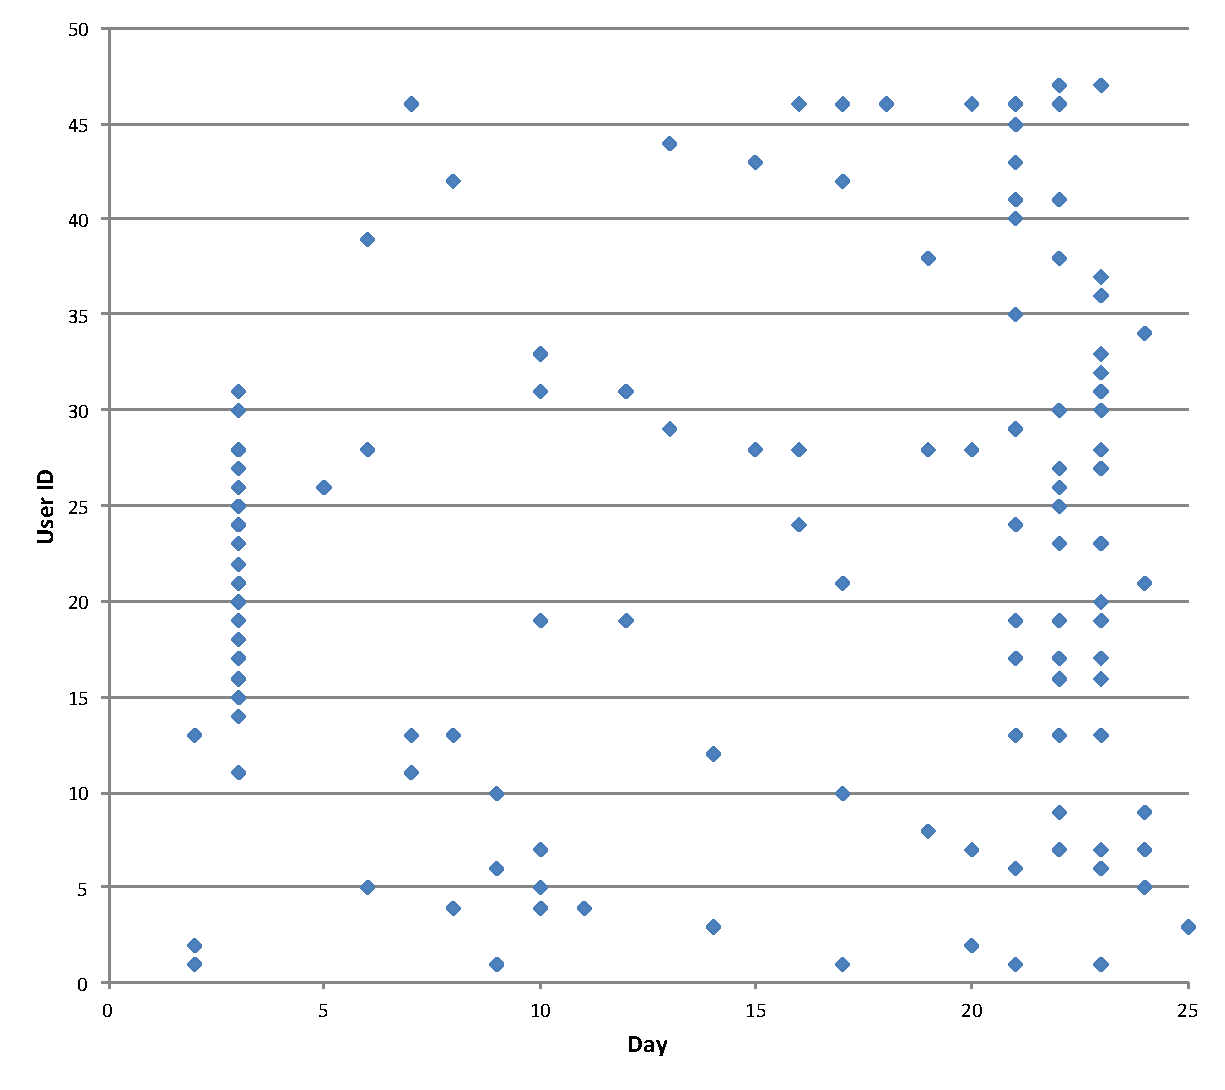
\includegraphics[width=0.8\columnwidth]{figures/user_exercise_activity_vs_day.pdf}
    \caption{The students are doing exercises at their own pace throughout the one month interval }
    \label{fig:activity_per_day}
  \end{figure}


% \begin{added}




\newpage
% \section{How Do Students Improve Their Vocabulary?}
% \section{How Does The System Help Students Improve Their Vocabulary?}
\section{What Is The Impact of the System on the Learner Vocabulary?}

  The value of extensive reading and vocabulary practice can be found, besides the new words that are learned, in the strengthening of the knowledge of the existing words, increased fluency, and increased grammar knowledge. Some of these benefits can only be clearly measured after a longer period of time\cite{renadya07-power}. 

  However, since our system combines free reading with vocabulary exercises, by analyzing the learner interaction with the reader and the exercises we can provide a glimpse into two measures of progress that are visible after one month of usage: strengthening knowledge of existing words and learning new ones. 

   \begin{figure}[h!]
  \centering
    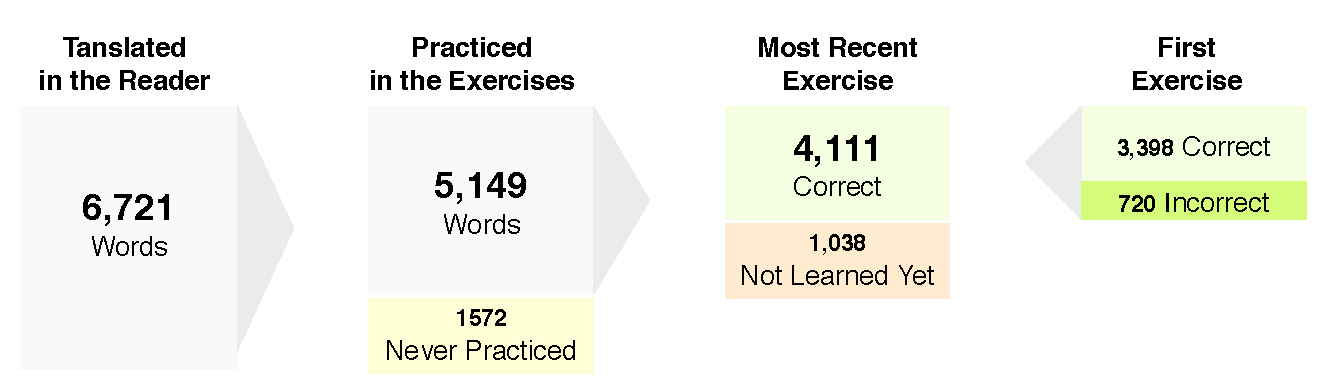
\includegraphics[width=0.9\columnwidth]{figures/word-learning-flow.pdf}
    \caption{An overview of the words encountered in the Reader and practiced in the Exercises}
    \label{fig:word_learning_flow}
  \end{figure}

   Looking at the outcomes of all the exercises done by the students we observe that:

  \begin{itemize}
    \item From the 6,721 words that were looked up in the reader, 5,149 were used in the exercises platform during the learning period. Since the learners requested a translation for these words we can assume that they were not known to the readers or at least the readers were unsure about their meaning. 

    \item More than 1,500 words were not practiced in the exercises. Some of these never got the chance to be scheduled by the algorithm and others were not presented to the students because the system decided they were not interesting enough. 
    % Given that not all the words can be practiced, this is an argument for prioritizing the words that the students are presented with in the exercises.

    \item For 80\% of the words that were present in exercises (4,111) the learners were able to correctly identify the meaning in the last associated exercise. Out of these: 

    \begin{itemize}
      \item 720 (14\%) of the words that were present in exercises were wrong during their first exercise interaction but were correct in the final one. These {\bf 720 words are likely to be learned via the exercises} by the sixty students in our study. They represent 10.75\% of all the words that the students translated in the reader.

      \item 66\% (3,398) were recognized already for the first time in the exercises. These are {\bf likely to be words for which the knowledge was strengthened by using the system}: the students were unsure when encountering them initially in the reader but eventually recognized their meaning when encountering them later in the exercises. 
    \end{itemize}

  \item For 20\% (1,038) of the words that were present in the exercises, the outcome of the final exercise that involved them showed an incorrect answer. Thus we can assume that they were {\bf not learned at the end of the experimental period}.

  \end{itemize}

% \end{added}














